\documentclass[dvipdfmx]{jsarticle}
\usepackage[T1]{fontenc}
\usepackage[dvipdfmx]{hyperref}
\usepackage{lmodern}
\usepackage{latexsym}
\usepackage{amsfonts}
\usepackage{amssymb}
\usepackage{mathtools}
\usepackage{amsthm}
\usepackage{multirow}
\usepackage{graphicx}
\usepackage{wrapfig}
\usepackage{here}
\usepackage{float}
\usepackage{ascmac}
\usepackage{url}

\title{オプション価格の決定-課題研究2-}
\author{文理学部情報科学科\\5419045 高林 秀}
\date{\today}

\begin{document}

\maketitle

\begin{abstract}
本稿は、疑似乱数とモンテカルロシミュレーションの考え利用して、今年度コンピューティング2の課題を解くものである。なお、本課題ではp5.jsを使用した。
\end{abstract}

\section{目的}
本稿は、今年度コンピューティング2の課題研究として「疑似乱数とモンテカルロシミュレーション」に関する問題に解答するものである。また同時に、問題に関する計算理論についても復習するものとする。
\section{計算理論}
\subsection{疑似乱数}
まず、乱数とはなにかについて説明する。乱数とは「ランダムな数こと」である。より厳密には、今得られている数列から、次の数列の値が予測できないような、いわゆる乱数列の各要素のことを乱数という。\par
コンピュータ上では乱数は様ざなま場面で利用されている。しかし、我々の知るコンピュータは決定性のある計算機であるため、コンピュータが乱数を生成するときはある計算法によって乱数を算出している。このように、コンピュータ上で実現される乱数を「擬似乱数」と呼ぶ。擬似乱数は、人間から見たときにランダムに値を生成するのであって、実際はある計算から導き出された値を使用している。\par
このような擬似乱数の生成方法の一つとして「線形合同法」が挙げられる。
\subsubsection{線形合同法:Linear Congruential Generators}
擬似乱数生成のアルゴリズムの一つで、生成される乱数は下記式で示される。
\begin{center}
  \begin{align*}
    ・生成される乱数列をX_{0}, X_{1}, X_{2}...とし、この各要素は\\
    X_{n+1} = aX_{n} + b mod m
  \end{align*}
\end{center}
このとき、$a, b, m$は乱数列を決定するパラメーターとなる。このとき、各パラメーターは$a < m, b < m, a > 0, b \geq 0$である必要がある。
また、生成される乱数列の$x_{0}$は乱数の種、シード値(SEED)と呼ばれるパラメーターである。シード値は擬似乱数生成アルゴリズムで生成される乱数列を制御するためのパラメーターで、このシード値によって生成される乱数の結果が決定する。すなわち、シード値が同じならば、何度擬似乱数生成アルゴリズムを実行しても生成される乱数は同じになる。よって一般的には、実行時の時間等をシード値として乱数を生成している。\par
$X_{n}$を使用して、$Y_{L}以上Y_{U}未満の実数値Y_{n}$を生成するときは下記式を使用する。
\begin{center}
  \begin{align*}
    Y_{n} = \frac{X_{n}}{m}(Y_{U}-Y_{L})+Y_{L}
  \end{align*}
\end{center}
下記に、線形合同法の利点・欠点をまとめる。
\begin{table}[H]
  \begin{center}
    \caption{線形合同法のメリット・デメリット}
    \begin{tabular}{|c|c|} \hline
      メリット & デメリット \\ \hline
      ・アルゴリズムの実装が簡単 & ・生成される乱数列に規則性がある\\
      ・生成が高速 & \\ \hline
    \end{tabular}
    \label{hyo01}
  \end{center}
\end{table}
線形合同法のアルゴリズムは非常にシンプルであるため、実装は用意である特徴を持つ。これは、先に示した計算式によって実装できるのが理由である。
以下、p5.jsにおける線形合同法の実装例を示す。各パラメーター値は$a = 5, b = 3, m = 16$である。
\begin{verbatim}
  let seed = 1;

function rand() {
  const a = 5;
  const b = 3;
  const m = 16;
  seed = (a * seed + b) % m;

  return seed;
}

function setup() {
  createCanvas(300, 300);
  noLoop();
}

function draw() {
  background(255);
  const repeat = 20;
  fill(0);
  textAlign(LEFT, TOP);
  for (let i = 0; i < repeat; ++i) {
    text(rand(), 0, 15 * i);
  }
}
\end{verbatim}
デメリットとして、生成される乱数に規則性がある。これは、線形合同法がもつ周期性に起因するものである。この線形合同法は最大で、$m$通りの乱数(整数値)を生成することができるが、前述したパラメーターの値により、生成する乱数の種類を$m$種類より小さくなるという問題がある。例えば、各パラメーターを$a = 7, b = 3, m = 16$としたとき、生成される乱数列は,$10, 9, 2, 1, 10, 9, 2, 1, 10, 9, 2, 1....$となり、出現する数字は$10, 9, 2, 1$の4通りとなる。この場合、4回ごとに生成される乱数列が1周していることになるので、このときの周期は4となる。一般的に、乱数の周期は長いほうがより望ましいため、線形合同法を使用するときはパラメーターの値によって周期が変化することに注意しなければならない。\par
線形合同法のパラメーター$m$は一般的に、$m = 2^{32} = 4294967296$とすることが知られている。なお、線形合同法は周期性を伴うので、より予測が困難な乱数列を利用したい場合は「メルセンヌ・ツイスタ」等の手法の利用が考えられる。
\subsection{モンテカルロシミュレーション}
モンテカルロシミュレーションとは「乱数を用いた試行を十分な回数繰り返すことで計算機の統計的な結果を得る」シュミュレーション方法である。別名モンテカルロ法とも呼ばれ、確率的な事象の推定値を得る場合に特にモンテカルロシュミュレーションと呼ばれる。\par
第二次世界大戦中、米ロスアラモス国立研究所で原子爆弾開発計画に従事していた核物理学者のスタニスワフ・ウラム(Stanislaw Ulam)氏によって、モンテカルロ法の原型が考案され、その後数学者のジョン・フォン・ノイマン(John von Neumann)氏が開発した計算機ENIACにおいてその有効性を証明したという経歴がある。
\subsection{確率分布}
まず、確率変数について説明する。確率変数とは、どんな値になるかが確率的に決定する変数のことをいう。そして確率分布とは、確率変数がとる値と、その値を取る確率の対応する様子のことをいう。例として、1〜6の目が出るさいころを考える。この場合、1〜6の確率変数はそれぞれ、$\frac{1}{6}$の確率が対応しているので、確率分布と言える。\par
このとき、確率変数$X$が確率分布関数$F(x)$に従う、といった言い方をする。
\paragraph{確率密度関数}さいころの出目を$X$としたとき、この$X$を離散確率変数と呼ぶ。反対に、0以上1以下の一様乱数\footnote{特定区間において、数値が同確率で出現する確率分布関数に従う乱数のこと。例:さいころの出目1〜6はそれぞれ$\frac{1}{6}で出現する一様乱数である$、このように言うことができる。}を生成する場合、出力である$X$の値は連続的な分布になる。このようなとき、
\begin{center}
  連続型確率変数$X$に対し、$X$が$a以上b以下となる確率が、$積分を使用して以下の式のように与えられるとき、$f(x)$を確率密度関数と呼ぶ。
  \begin{align*}
    P(a \leq X \leq b) = \int^b_a f(x)dx
  \end{align*}
\end{center}
\paragraph{確率分布関数}確率変数がある値を取るときの確率分布を示した関数を確率分布関数と呼ぶ。確率分布関数は確率密度関数の積分によって定義される。\par
確率変数$X$が確率分布関数$F(x)$に従うことを、$X \simeq F(x)$と表記する。
なお、確率分布関数は$0 \leq F(x) \leq 1$である。
\subsubsection{正規分布}
正規分布とは、別名ガウス分布とも呼ばれ、平均値を中心に左右対称な山型の分布をする確率分布のことをいう。
\begin{figure}[H]
  \centering
  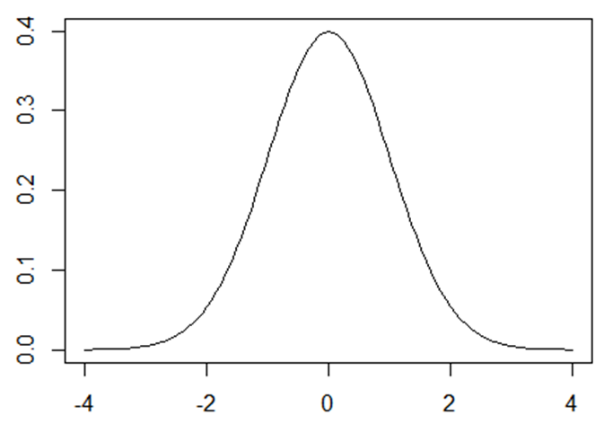
\includegraphics[scale=0.6]{795316b92fc766b0181f6fef074f03fa-8.png}
  \caption{正規分布の一例}
  \url{https://bellcurve.jp/statistics/course/7797.html}
\end{figure}
正規分布では、平均値から離れている値ほど、その正規確率も小さくなるようになっている。平均値が$\mu$、標準偏差が$\sigma$の正規分布を$N(\mu, \sigma^{2})$と記す。特に、平均$\mu = $0、標準偏差$\sigma = $1の正規分布を「標準正規分布」と呼ぶ。$X \simeq N(0, 1)とY \simeq N(\mu, \sigma^{2})の関係はY = \sigma X + \mu$となる。これは、任意の正規分布を作成するには、標準正規分布を作成すれば良いことを意味する。\par
\subsubsection{逆関数法}
確率変数$X$の確率分布関数$F(x)$が与えられているとき、$0 \leq F(x) \leq 1$であり、$F(x) = y$とすると、$-\infty からxまでの累積確率はy$となる。よって、$F(x)の逆関数F^{-1}(Y)によって確率分布関数F(x)に従う乱数を得ることができる。$これを逆関数法と呼ぶ。
\paragraph{一様分布に従う乱数の生成}
$a以上b未満の一様乱数をU(a,b)と表記するとき、U(a, b)の確率分布関数F(x)は次のようになる$。
\begin{center}
  \begin{align*}
    F(x) = \frac{x-a}{b-a} | a \leq x < b
  \end{align*}
\end{center}
\paragraph{指数分布に従う乱数の生成}
指数分布とは、連続型確率分布の1つであり、ある事象が発生してから次にその事象が発生するまでの期間が従う分布を表す。
\begin{figure}[H]
  \centering
  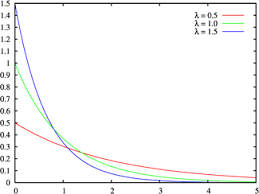
\includegraphics[scale=0.6]{sisuu.png}
  \caption{指数分布の一例}
  \url{https://ja.wikipedia.org/wiki/%E6%8C%87%E6%95%B0%E5%88%86%E5%B8%83}
\end{figure}
平均$\mu$の指数分布における確率密度関数は次のように示される。
\begin{center}
  \begin{align*}
    f(x) = \frac{1}{\mu}e^{-\frac{x}{\mu}} | x(0 \leq x)
  \end{align*}
\end{center}
このとき、事象の発生間隔が$Exp(\lambda )$に従うとしたとき、その発生間隔の期待値は$\frac{1}{\lambda}$となる。\par
なお、$Exp(\lambda)$の分布関数$F(x)$は次の通り。
\begin{center}
  \begin{align*}
    F(x) = 1-e^{-\lambda x}
  \end{align*}
\end{center}
であり、その逆関数は、
\begin{center}
  \begin{align*}
    F^{-1}(x) = -\frac{\log(1-x)}{\lambda}
  \end{align*}
\end{center}
\paragraph{正規分布に従う乱数の生成}
正規分布の分布関数の逆関数は求めることができない。\par
そこでまず、標準正規分布の分布関数を2次元で図示したときの上から見た図(下図)上の任意の点$(x,y)$における、原点(0, 0)との距離$R$と、2点を結ぶん辺のなす角を$\theta$とする。\par
このとき正規分布は独立な確率変数$R \simeq Exp(2), \theta \simeq U(0, 2\pi)$で次のように示すことができる。
\begin{center}
  \begin{align*}
    N(0, 1) = \sqrt{R}cos\theta
  \end{align*}
\end{center}
これは、$R, \theta$を得ることができれば、標準正規分布を得ることができることを意味している。これを、Box-Muller法と呼ぶ。
\paragraph{Poisson分布(ポアソン分布)に従う乱数の生成}
Poisson分布とは、単位時間あたり平均して$\lambda$回生起する事象が、単位時間に$k$回生起する確率を示すのに使用される確率分布のことを意味する。この様な事象は一般的に、下記式で示されることが知られている。
\begin{center}
  \begin{align*}
    P(k) = \frac{\lambda^{k}e^{-\lambda}}{k!}
  \end{align*}
\end{center}
特に、確率変数$X$が上記式を満たしているとき、確率変数$X$はパラメータ$\lambda$のPoisson分布に従っている、という。
\begin{figure}[H]
  \centering
  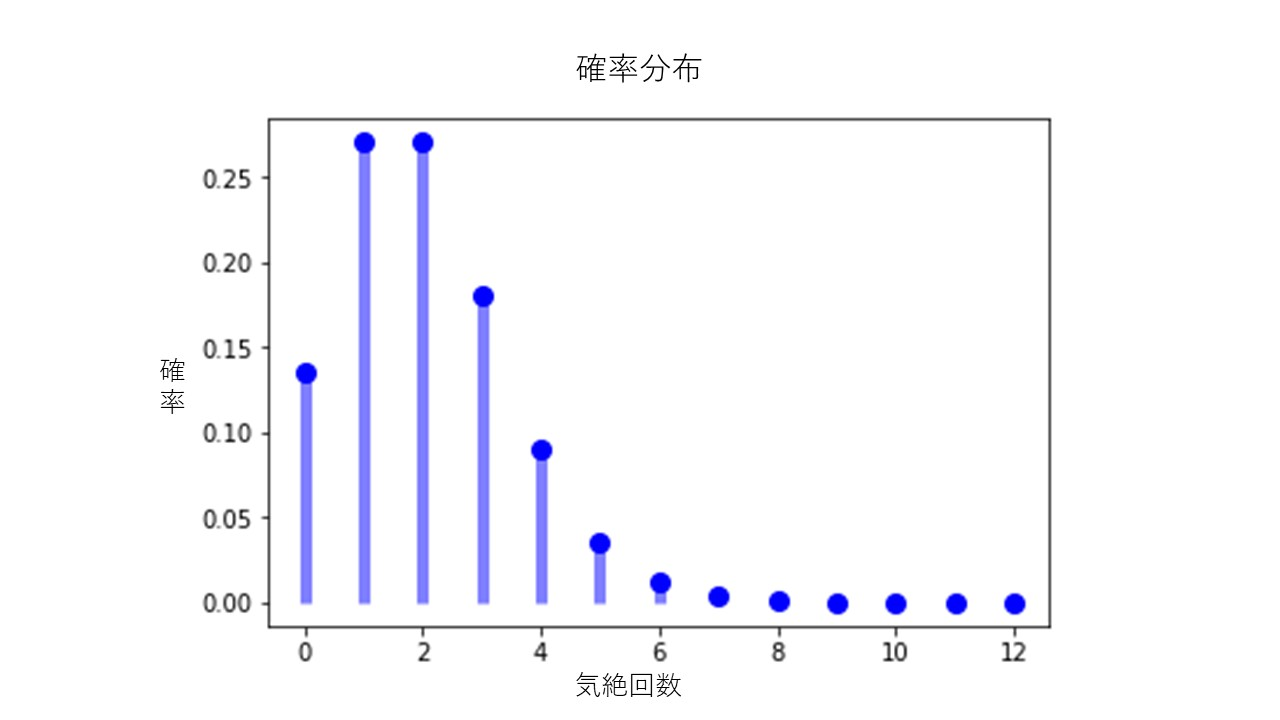
\includegraphics[scale=0.3]{poi_fig_1.jpg}
  \caption{Poisson分布の一例}
  \url{https://recruit.cct-inc.co.jp/tecblog/machine-learning/poisson/}
\end{figure}
ある事象が、時間的に一様に生起する時、単位時間あたりその事象の生起回数は、Poisson分布に従うことが知られている。Poisson分布の確率分布を$Po(\lambda)$とするとき、その期待値は$\lambda$になる。\par
Poisson分布に従った乱数は、指数分布$Exp(\lambda)$を用いて生成することができる。つまり、指数分布に従っている事象が一定間隔に何回生起したか数えることによりPoisson分布に従った乱数を生成することができる。なお、Poisson分布は離散的な確率分布であることに留意する必要がある。\par

p5.jsでは、$randomGaussian()$関数によって、標準正規分布に従う乱数列を生成することができるが、上記に列挙した標準正規分布以外の分布で乱数列を生成するときは自身でコードを作成し、実装する必要がある。
\subsection{ランダムウォーク}
ある値が、一定時間ごとに過去の状態に依存せず、ランダムに変動するような事象をランダムウォークと呼ぶ。ある値、$SがS_{0}から始まり、時刻i-1とiの間のSの変化量確率変数X_{i}\simeq Fと示されるとき、時刻tにおけるS値S_{t}は次のように示すことができる。$
\begin{center}
  \begin{align*}
    S_{t} = S_{0} + \Sigma_{i=1}^{t}X_{i}
  \end{align*}
\end{center}
ランダムウォークは、ブラウン運動\footnote{微粒子が分子と衝突した際に起きる不規則な運動のこと}等の物理現象と結び付けられて解析が行われることが多い。その他にも、株価の変動をランダムウォークとみなし、利益や損失の推定を行うことがある。

ランダムウォークは、異なる時点$i, j$における確率変数$X_{i}, X_{j}$は独立であるという特徴を持つ。この時、$X_{i}の期待値E|X_{i}| = \mu 、分散をV|X_{i}| = \sigma^{2}$で示すと、$S_{t}における期待値とその分散は次のようになる$。
\begin{center}
  \begin{align*}
    E|S_{t}| = S_{0} + t\mu \\
    V|S_{t}| = t\sigma^{2}
  \end{align*}
\end{center}
\section{実験方法}
\subsection{計算機環境}
本課題を解いた際の計算機環境を下記に示す。
\begin{itemize}
  \item ホストOS:Window10 Home Ver.20H2
  \item 仮想OS:Ubuntu 20.04.2 LTS
  \item CPU:Intel(R)Core(TM)i7-9700K @ 3.6GHz
  \item GPU:Nvidia Geforce RTX2070 OC @ 8GB
  \item ホストRAM:16GB
  \item 仮想RAM:4GB
\end{itemize}
\subsection{課題}
現在A社の株価は10000円である。A社のかk部下は毎日正規分布$N(5, 200^{2})$に従って変動する。365日後にこの株を、株価の変動によらず10000で買う権利をオプjションと呼ぶ。買い手は売り手からこのオプションを手数料$X$円で購入する。例えば、365日後に株価が12000円となった場合、オプション行使することで差額から手数料を引いた$2000-X$円だけ書いては得をする。このとき売り手は$X-2000$円の損をする、また、365日後に株価が8000円となった場合、オプションを行使しないことで買い手の損失は手数料の$X$円分だけでよくなる。このとき売り手は$X$円の損をする。
\begin{table}[H]
  \begin{center}
    \begin{tabular}{|c|c|c|} \hline
      365日後の株価の変動$Y$ & 買い手の損得(円) & 売り手の損得(円) \\ \hline
      $Y > 0$ & $Y - X$ & $X - Y$ \\
      $Y \leq 0$ & $-X$ & $X$ \\ \hline
    \end{tabular}
    \label{hyo02}
  \end{center}
\end{table}
\paragraph{Q1}365日後の株価の期待値をモンテカルロシミュレーションによって求めよ。
\paragraph{Q2}Q1で得られた株価の変動について十分な回数試行を行い365日後の株価のヒストグラムを画面に描画せよ。
\paragraph{Q3}売り手が収入の期待値がマイナスにならないようにコールオプションを販売するとき、コールオプションの価格はいくらにすれば良いか、モンテカルロシミュレーションを用いて検討せよ。
\section{結果と考察}
\paragraph{Q1}
下記に添付したJavaScript(p5.js)よって求めた。その結果を以下に示す。
\begin{itemize}
  \item Q1.js : \url{}
\end{itemize}
\section{まとめ}
\section{付録}

\end{document}
